\documentclass[10pt,a4paper]{article}

\usepackage[margin=19mm,top=17mm,bottom=20mm]{geometry}
\usepackage[T1]{fontenc}
\usepackage{lmodern}
\usepackage{microtype}
\usepackage{amsmath}
\usepackage{booktabs}
\usepackage{tabularx}
\usepackage{graphicx}
\usepackage{float}
\usepackage{placeins}
\usepackage{xcolor}
\usepackage{tikz}
\usetikzlibrary{arrows.meta,positioning}
\usepackage{enumitem}
\usepackage[font=small,labelfont=bf]{caption}
\usepackage{titlesec}
\usepackage[hidelinks]{hyperref}

\definecolor{reportteal}{HTML}{087F8C}
\definecolor{reportblue}{HTML}{286F9B}
\definecolor{reportorange}{HTML}{D97706}
\hypersetup{colorlinks=true,linkcolor=reportteal,citecolor=reportteal,urlcolor=reportblue}

\titleformat{\section}[block]{\large\bfseries}{\thesection}{0.55em}{}
\titleformat{\subsection}[block]{\normalsize\bfseries}{\thesubsection}{0.5em}{}
\titlespacing*{\section}{0pt}{1.0ex plus 0.4ex}{0.45ex}
\titlespacing*{\subsection}{0pt}{0.75ex plus 0.3ex}{0.3ex}
\setlist{nosep,leftmargin=1.4em}
\setlength{\parindent}{0pt}
\setlength{\parskip}{0.45ex}
\setlength{\textfloatsep}{8pt plus 2pt minus 2pt}
\setlength{\floatsep}{7pt plus 2pt minus 2pt}
\setlength{\intextsep}{7pt plus 2pt minus 2pt}

\newcommand{\LaneGroup}{\textsc{LaneGroup}}
\newcommand{\Movement}{\textsc{Movement}}

\title{\vspace{-1.8em}\textbf{A Graph-Based Control Interface for Traffic Signals\\on Heterogeneous Road Networks}}
\author{Bertil Braun}
\date{}

\begin{document}
\maketitle
\vspace{-2.2em}

\begin{abstract}
We present a traffic-signal control interface in which a shared graph neural network assigns scores to individual traffic movements.
Each junction converts these scores into its own variable-sized set of legal signal phases using a deterministic incidence matrix.
Directed corridor nodes provide traffic context, while movement nodes represent controlled input-to-output paths through junctions.
Typed mean aggregation produces one scalar per movement; phase definitions and signal timing remain outside the learned network.
This makes graph size and junction-specific action count independent of the learned parameter shapes.
PPO experiments provide a feasibility evaluation: three trained policies were evaluated on unseen synthetic grid sizes and aspect ratios, signal-coverage changes exposed a distribution-shift limitation, and one trained parameter instance executed on five heterogeneous city graphs.
The evidence supports the implemented interface and reports the outcomes of the evaluated runs, rather than establishing general transfer across arbitrary road networks.
\end{abstract}

\section{Introduction}

Traffic-signal action spaces are local.
A three-arm junction, a regular four-arm junction, and a junction with protected turns need not have the same number or meaning of phases.
Consequently, a fixed output called ``phase 2'' does not have reusable semantics across road networks.

We present a traffic-signal control interface in which a shared graph neural network assigns scores to individual traffic movements.
Each junction converts these scores into its own variable-sized set of legal signal phases using a deterministic incidence matrix.
The central design choice is therefore a narrow boundary: learning prioritizes comparable movement objects, while deterministic code constructs and operates each junction's valid local choices.

The report makes three contributions:
\begin{enumerate}
  \item a reusable movement-level graph representation with directed corridor context;
  \item deterministic construction of junction-specific action spaces and movement-to-phase mapping; and
  \item an empirical feasibility evaluation across synthetic grids, signal-coverage conditions, and heterogeneous city simulations.
\end{enumerate}

The evaluation is organized around four research questions:
\begin{description}[leftmargin=4.2em,style=nextline]
  \item[RQ1 --- Structural applicability.] Can one learned parameterization operate on networks with different graph sizes and junction-specific phase counts?
  \item[RQ2 --- Synthetic transfer.] How does the trained policy behave on unseen grid sizes and aspect ratios produced by the same generator?
  \item[RQ3 --- Distribution shift.] What happens when signal coverage changes?
  \item[RQ4 --- City feasibility.] Can the same trained policy execute on several heterogeneous city simulations, and how variable are the observed outcomes?
\end{description}
RQ1 is answered primarily by the construction and verified by execution; RQ2--RQ4 require empirical evidence.

Movement pressure and movement-structured control have substantial prior lineage.
Max-pressure methods score compatible stages from constituent flows \cite{varaiya2013maxpressure}; PressLight connects pressure to learned control \cite{wei2019presslight}; and FRAP represents phase competition through movements \cite{zheng2019frap}.
TransferLight also maps movement representations to variable phase spaces, using a learned hierarchical phase encoder \cite{schmidt2024transferlight}.
The contribution here is the transparent interface between a city-level typed graph, scalar movement scores, and conflict-derived local matrices.

\textbf{Scope.}
This report evaluates an implementation and architectural interface rather than proposing a new reinforcement-learning algorithm.
The experiments test whether one parameterization can execute across heterogeneous action spaces and provide preliminary evidence of transfer within the evaluated simulation families.
They do not establish general transfer across arbitrary road networks.

\section{Movement-level control interface}

\subsection{Intuition and control objects}

A \emph{movement} is one legal controlled path from an incoming road corridor to an outgoing corridor; straight travel is a movement as well as a turn.
A \emph{phase} is a compatible set of movements that may receive green together.
The controller chooses one phase per junction, rather than setting individual lamps independently.

\begin{figure}[H]
  \centering
  \resizebox{\linewidth}{!}{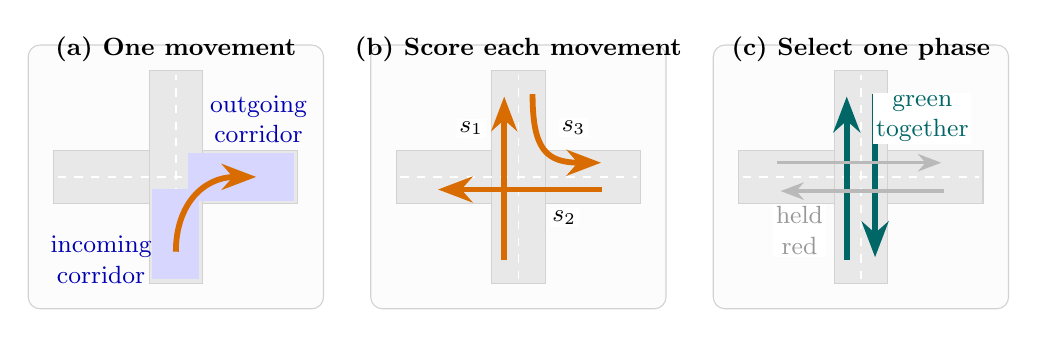
\begin{tikzpicture}[
  x=1cm,
  y=1cm,
  panel/.style={
    draw=gray!35,
    rounded corners=1.5mm,
    fill=gray!2,
    minimum width=3.75cm,
    minimum height=3.35cm
  },
  road/.style={fill=gray!18, draw=gray!35},
  movement/.style={->, >=Stealth, line width=2.1pt, color=orange!85!black},
  active/.style={->, >=Stealth, line width=2.2pt, color=teal!80!black},
  inactive/.style={->, >=Stealth, line width=1.2pt, color=gray!55},
  label/.style={font=\small, align=center}
]
  \foreach \offset in {0,4.35,8.7} {
    \begin{scope}[xshift=\offset cm]
      \node[panel] at (0,0) {};
      \path[road] (-1.55,-0.34) rectangle (1.55,0.34);
      \path[road] (-0.34,-1.35) rectangle (0.34,1.35);
      \draw[white, line width=0.6pt, dashed] (-1.5,0) -- (1.5,0);
      \draw[white, line width=0.6pt, dashed] (0,-1.3) -- (0,1.3);
    \end{scope}
  }

  \begin{scope}
    \path[fill=blue!16] (-0.30,-1.30) rectangle (0.30,-0.15);
    \path[fill=blue!16] (0.15,-0.30) rectangle (1.50,0.30);
    \draw[movement] (0,-0.95) .. controls (0,-0.35) and (0.35,0) .. (1.02,0);
    \node[label, text=blue!70!black] at (-0.95,-1.05) {incoming\\corridor};
    \node[label, text=blue!70!black] at (1.05,0.73) {outgoing\\corridor};
    \node[font=\small\bfseries] at (0,1.62) {(a) One movement};
  \end{scope}

  \begin{scope}[xshift=4.35cm]
    \draw[movement] (-0.18,-1.05) -- (-0.18,1.02);
    \draw[movement] (1.06,-0.16) -- (-1.02,-0.16);
    \draw[movement] (0.18,1.05) .. controls (0.18,0.35) and (0.35,0.18) .. (1.05,0.18);
    \node[label, fill=white, inner sep=1pt] at (-0.60,0.62) {$s_1$};
    \node[label, fill=white, inner sep=1pt] at (0.58,-0.52) {$s_2$};
    \node[label, fill=white, inner sep=1pt] at (0.70,0.63) {$s_3$};
    \node[font=\small\bfseries] at (0,1.62) {(b) Score each movement};
  \end{scope}

  \begin{scope}[xshift=8.7cm]
    \draw[active] (-0.18,-1.05) -- (-0.18,1.02);
    \draw[active] (0.18,1.05) -- (0.18,-1.02);
    \draw[inactive] (-1.06,0.18) -- (1.02,0.18);
    \draw[inactive] (1.06,-0.18) -- (-1.02,-0.18);
    \node[label, text=teal!80!black, fill=white, inner sep=1pt] at (0.78,0.74)
      {green\\together};
    \node[label, text=gray!80, fill=white, inner sep=1pt] at (-0.78,-0.68)
      {held\\red};
    \node[font=\small\bfseries] at (0,1.62) {(c) Select one phase};
  \end{scope}
\end{tikzpicture}
}
  \caption{The control vocabulary. The shared model scores movements individually; each junction supplies its own compatible phase sets. The phase shown is illustrative, not a universal template.}
  \label{fig:concepts}
\end{figure}
\FloatBarrier

The implementation groups consecutive directed road segments into a \LaneGroup{} when an unsignalized continuation is unambiguous.
Opposite directions remain separate because their queues, speeds, and destinations differ.
At a controlled junction, a legal input-to-output connection becomes a \Movement{} node.
The junction owns its Movements and phases but is not itself a GNN node.

\begin{table}[H]
  \small
  \centering
  \caption{Roles in the representation and action interface.}
  \begin{tabularx}{\linewidth}{@{}lXX@{}}
    \toprule
    Object & Represents & Used for\\
    \midrule
    \LaneGroup & One direction of a road corridor & Queue, speed, occupancy, capacity, arrivals, departures, and downstream space\\
    \Movement & One controlled input-to-output path & Turn-local demand, controlled-link count, and recent green state\\
    Phase & One compatible local Movement set & A junction-specific selectable action\\
    \bottomrule
  \end{tabularx}
  \label{tab:terminology}
\end{table}

At each decision, features are refreshed from SUMO, the shared GNN emits one score per Movement, and a junction-local incidence matrix converts those scores to phase logits.
An availability mask enforces minimum green; the runtime inserts yellow when an accepted target changes.
Only movement scoring is learned.

\subsection{Typed graph and exact message passing}

Each Movement \(m\) has one input LaneGroup \(i(m)\) and one output LaneGroup \(o(m)\), giving four directed information relations:
\[
L_{\mathrm{in}}\!\rightarrow M,\quad
L_{\mathrm{out}}\!\rightarrow M,\quad
M\!\rightarrow L_{\mathrm{in}},\quad
M\!\rightarrow L_{\mathrm{out}}.
\]
The output-to-movement relation returns downstream storage context to a movement that would feed that corridor.
Unsignalized pass-through connections are weighted \(L\!\rightarrow L\) edges with \(w_{ql}=\exp(-t_{\mathrm{ff}}/30\,\mathrm{s})\).

Let \(\rho\) denote ReLU, \(\Vert\) concatenation, and \(x_l,x_m\) the LaneGroup and Movement feature vectors.
The implementation first creates
\begin{align}
h_l^{(0)} &= \rho(E_Lx_l),\\
h_m^{(0)} &= \rho\!\left(E_M[x_m\Vert h_{i(m)}^{(0)}\Vert h_{o(m)}^{(0)}]\right).
\end{align}
For relation \(r\), target \(v\), and source embeddings \(z_q\), define the implemented transformed mean
\[
\mathcal A_r^{(k)}(v;z)=
\frac{1}{\max(1,|\mathcal N_r(v)|)}
\sum_{q\in\mathcal N_r(v)} w_{qv}W_r^{(k)}z_q,
\]
where \(w_{qv}=1\) except on unsignalized connector edges; an empty neighbourhood produces zero.
One block updates Movements first and then LaneGroups:
\begin{align}
h_m^{(k+1)}={}&\rho\!\left(U_M^{(k)}\left[
h_m^{(k)}\Vert
\mathcal A_{L_{\mathrm{in}}\to M}^{(k)}(m;h_L^{(k)})\Vert
\mathcal A_{L_{\mathrm{out}}\to M}^{(k)}(m;h_L^{(k)})
\right]\right),\label{eq:movement-update}\\
h_l^{(k+1)}={}&\rho\!\left(U_L^{(k)}\left[
h_l^{(k)}\Vert
\left(\mathcal A_{M\to L_{\mathrm{in}}}^{(k)}(l;h_M^{(k+1)})+
\mathcal A_{L\to L}^{(k)}(l;h_L^{(k)})\right)\Vert
\mathcal A_{M\to L_{\mathrm{out}}}^{(k)}(l;h_M^{(k+1)})
\right]\right).\label{eq:lane-update}
\end{align}
Thus every relation has its own linear map, aggregation is a mean rather than attention, and reverse Movement messages use the just-updated embeddings from \eqref{eq:movement-update}.
After two blocks, an MLP maps every \(h_m^{(2)}\) to one scalar \(s_m\).
The critic mean-pools the Movement embeddings owned by each junction and returns one value per controller.

\begin{figure}[H]
  \centering
  \resizebox{\linewidth}{!}{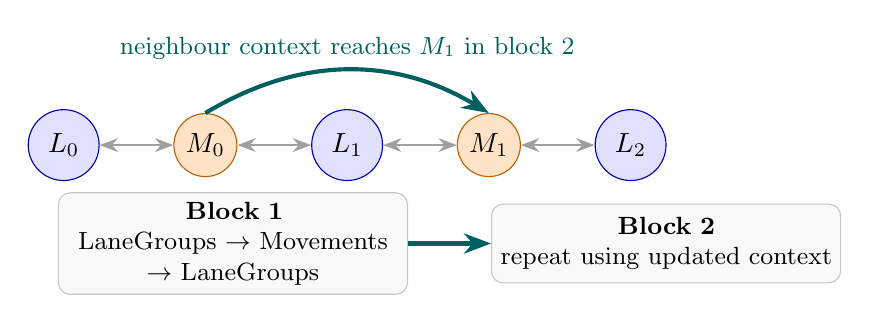
\begin{tikzpicture}[
  x=1cm,
  y=1cm,
  lane/.style={circle, draw=blue!65!black, fill=blue!12, minimum size=9mm, inner sep=0pt},
  movement/.style={circle, draw=orange!75!black, fill=orange!22, minimum size=8mm, inner sep=0pt},
  relation/.style={<->, >=Stealth, line width=0.8pt, color=gray!75},
  influence/.style={->, >=Stealth, line width=1.5pt, color=teal!75!black},
  block/.style={
    draw=gray!45,
    rounded corners=1.5mm,
    fill=gray!5,
    text width=4.2cm,
    minimum height=10mm,
    font=\small,
    align=center
  },
  note/.style={font=\small, align=center}
]
  \node[lane] (l0) at (0,0) {$L_0$};
  \node[movement] (m0) at (1.8,0) {$M_0$};
  \node[lane] (l1) at (3.6,0) {$L_1$};
  \node[movement] (m1) at (5.4,0) {$M_1$};
  \node[lane] (l2) at (7.2,0) {$L_2$};

  \draw[relation] (l0) -- (m0);
  \draw[relation] (m0) -- (l1);
  \draw[relation] (l1) -- (m1);
  \draw[relation] (m1) -- (l2);

  \draw[influence, bend left=31] (m0.north) to
    node[above, note] {neighbour context reaches $M_1$ in block 2}
    (m1.north);

  \node[block] (block1) at (2.15,-1.25)
    {\textbf{Block 1}\\LaneGroups $\rightarrow$ Movements\\$\rightarrow$ LaneGroups};
  \node[block] (block2) at (7.65,-1.25)
    {\textbf{Block 2}\\repeat using updated context};
  \draw[influence] (block1.east) -- (block2.west);
\end{tikzpicture}
}
  \caption{The typed representation and update order. With this order, two blocks allow information from one Movement to reach another through a shared LaneGroup. The experiments evaluate the resulting two-block architecture but do not isolate the contribution of depth.}
  \label{fig:representation}
\end{figure}
\FloatBarrier

The parameter matrices above are shared over all nodes and edges of a type.
Their shapes depend on feature and hidden dimensions, not on node count, Movement count, or phase count.
This is an architectural property, not an empirical transfer claim.

\subsection{Deterministic local action spaces}

The build pipeline obtains controlled links and request-conflict data from SUMO \texttt{netconvert} \cite{alvarezlopez2018sumo}.
Links constrained to activate together form atomic groups; groups with internal SUMO conflicts are rejected.
Two groups are incompatible when SUMO reports a conflict in either direction or different incoming approaches merge into the same outgoing edge.
Bron--Kerbosch enumeration \cite{bron1973cliques} produces all maximal compatible group sets, each of which becomes a selectable phase.
Here, maximal means that no additional compatible group can be added, not that the phase has maximum size.

For junction \(j\), \(A_j\in\{0,1\}^{|P_j|\times|M_j|}\) records whether phase \(p\) enables Movement \(m\).
The local logits are
\[
\boldsymbol\ell_j=A_j\mathbf s_j,
\qquad
\ell_{j,p}=\sum_{m\in M_j}A_{j,p,m}s_m.
\]
For example,
\[
A_j=
\begin{bmatrix}1&1&0&0\\0&0&1&1\end{bmatrix},\qquad
\mathbf s_j=
\begin{bmatrix}1.2&0.7&0.6&-0.4\end{bmatrix}^{\mathsf T},\qquad
A_j\mathbf s_j=
\begin{bmatrix}1.9&0.2\end{bmatrix}^{\mathsf T}.
\]
The first phase receives the larger logit; masking and categorical sampling follow before the runtime applies any signal transition.
A different junction may provide a \(6\times11\) matrix without changing the scorer.

\begin{figure}[H]
  \centering
  \resizebox{\linewidth}{!}{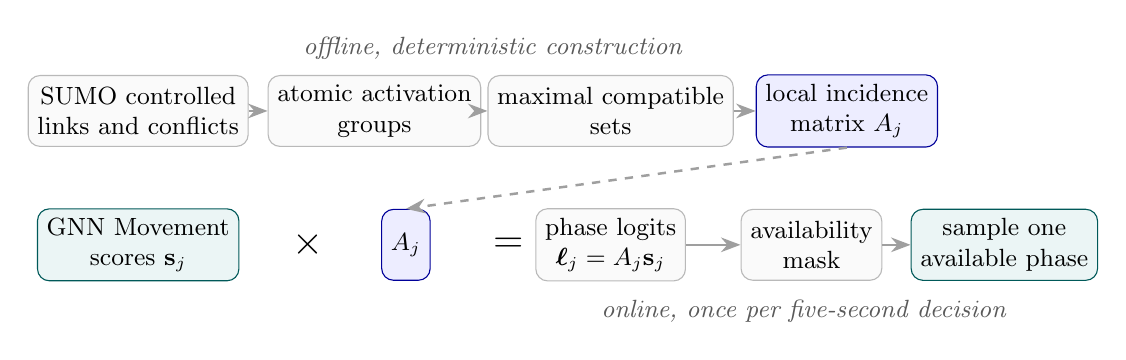
\begin{tikzpicture}[
  x=1cm,
  y=1cm,
  box/.style={draw=gray!55, rounded corners=1.5mm, fill=gray!4, minimum height=9mm, align=center, font=\small},
  arrow/.style={->, >=Stealth, line width=0.9pt, color=gray!75},
  learned/.style={draw=teal!70!black, fill=teal!8},
  fixed/.style={draw=blue!60!black, fill=blue!7}
]
  \node[box] (links) at (0,1.2) {SUMO controlled\\links and conflicts};
  \node[box] (groups) at (3.0,1.2) {atomic activation\\groups};
  \node[box] (cliques) at (6.0,1.2) {maximal compatible\\sets};
  \node[box, fixed] (incidence) at (9.0,1.2) {local incidence\\matrix $A_j$};
  \draw[arrow] (links) -- (groups);
  \draw[arrow] (groups) -- (cliques);
  \draw[arrow] (cliques) -- (incidence);
  \node[font=\small\itshape, text=gray!70!black] at (4.5,2.0) {offline, deterministic construction};

  \node[box, learned] (scores) at (0,-0.5) {GNN Movement\\scores $\mathbf{s}_j$};
  \node[font=\Large] at (2.15,-0.5) {$\times$};
  \node[box, fixed] (matrixcopy) at (3.4,-0.5) {$A_j$};
  \node[font=\Large] at (4.7,-0.5) {$=$};
  \node[box] (logits) at (6.0,-0.5) {phase logits\\$\boldsymbol{\ell}_j=A_j\mathbf{s}_j$};
  \node[box] (mask) at (8.55,-0.5) {availability\\mask};
  \node[box, learned] (action) at (11.0,-0.5) {sample one\\available phase};
  \draw[arrow] (logits) -- (mask);
  \draw[arrow] (mask) -- (action);
  \draw[arrow, dashed] (incidence.south) -- (matrixcopy.north);
  \node[font=\small\itshape, text=gray!70!black] at (8.45,-1.35) {online, once per five-second decision};
\end{tikzpicture}
}
  \caption{Offline phase construction and online action selection. The fixed incidence matrix changes with each junction; the learned scorer does not.}
  \label{fig:phase-interface}
\end{figure}
\FloatBarrier

Sum aggregation is an additive inductive bias: when Movement scores are positive, a phase containing more Movements can receive a larger logit simply because it has more terms.
This phase-size effect was not evaluated separately.

\section{Experimental design and reproducibility}

\subsection{Training protocol and local reward}

PPO \cite{schulman2017ppo} optimizes the complete policy.
All reported studies use two message-passing blocks, \(5\,\mathrm{s}\) decisions, immediate \(3\,\mathrm{s}\) yellow on a change, one decision of minimum green, four PPO epochs, 200 decisions per rollout, and entropy coefficient \(0.001\).
Rollout counts are allocated to approximately balance junction/action samples across differently sized training graphs.

The code assigns one reward to each junction \(j\) per decision interval \(\Delta=5\,\mathrm{s}\).
Let \(I_j\) be its unique incoming lanes, \(D_j=\sum_{l\in I_j}D_l\) their total length, \(n_l\) the vehicle count, \(\bar v_l\) mean speed, \(v_l^{\max}\) speed limit, and \(V_j(t)\) the set of vehicle IDs on those lanes.
With \(f_l(t)=\operatorname{clip}(\bar v_l(t)/v_l^{\max},0,1)\), the implemented terms are:

\begin{table}[H]
  \footnotesize
  \centering
  \caption{Exact local reward terms for the reported runs. Values are sampled at decision boundaries.}
  \begin{tabularx}{\linewidth}{@{}lXl@{}}
    \toprule
    Term & Definition and interpretation & Unit\\
    \midrule
    Progress \(p_j\) & \(D_j^{-1}\sum_{l\in I_j}n_l(t)f_l(t)\): speed-normalized moving-vehicle density & veh/m\\
    Discharge \(d_j\) & \(|V_j(t-\Delta)\setminus V_j(t)|/(\Delta D_j)\): IDs leaving the incoming-lane set & veh/(m\,s)\\
    Braking \(b_j\) & \((\Delta D_j)^{-1}\sum_{l\in I_j}n_l(t)[\bar v_l(t-\Delta)-\bar v_l(t)]_+/v_l^{\max}\) & veh/(m\,s)\\
    Gridlock \(q_j\) & \(D_j^{-1}\sum_{l\in I_j}n_l(t)(1-f_l(t))\): speed-deficit density & veh/m\\
    \bottomrule
  \end{tabularx}
  \label{tab:reward}
\end{table}

The first braking sample is zero because no preceding snapshot exists.
The per-junction reward is
\[
r_j=\operatorname{clip}_{[-1,1]}\!\left(p_j+10d_j-10b_j-0.02q_j\right).
\]
Global delay, completed-network flow, direct throughput, phase switching, and teleport terms have zero weight in these runs.
The displayed units therefore describe the normalized inputs; the weighted sum is an engineered scalar objective rather than a physical quantity.

\subsection{Evaluation metrics}

Every episode records per-seed metrics before arithmetic means are formed.
For an episode of \(T\) simulated seconds, let \(C\) be trips with a SUMO \texttt{tripinfo} arrival after warm-up and \(D\) the initial post-warm-up population plus subsequent departures.

\begin{table}[H]
  \footnotesize
  \centering
  \caption{Primary evaluation metrics and aggregation.}
  \begin{tabularx}{\linewidth}{@{}lXl@{}}
    \toprule
    Metric & Implemented definition & Unit\\
    \midrule
    Throughput & \(C/(T/3600)\) & veh/h\\
    Completion & \(C/D\); vehicles still active at the horizon remain incomplete & fraction or \%\\
    Completed-trip wait & Mean SUMO \texttt{waitingTime} over the \(C\) completed trips & s\\
    Wait density & Time mean of \(\sum_l W_l(t)/\sum_l D_l\), where \(W_l\) is SUMO's total waiting time of vehicles currently on lane \(l\) & s/m\\
    \bottomrule
  \end{tabularx}
  \label{tab:metrics}
\end{table}

Wait density uses all non-internal network lanes at every simulated second and exposes queues left at the horizon; completed-trip waiting excludes unfinished vehicles.
Grid results separate three policy-training seeds from six fresh traffic seeds.
The city evaluation has one policy-training seed and three traffic seeds per city, so its dispersion does not estimate training-run variability.

\subsection{Baseline protocol and study matrix}

All policies receive the same saved SUMO network, routes, initial-occupancy range, warm-up, episode seed, conflict-derived phase set, minimum-green rule, and yellow transition.
The learned and uniform-random policies choose every \(5\,\mathrm{s}\); fixed time cycles through phase order every \(10\,\mathrm{s}\); max pressure and queue recompute a target every \(10\,\mathrm{s}\).
Max pressure observes the instantaneous halting counts in the downstream detector regions of the Movement's input and output LaneGroups and scores \(n^{\mathrm{halt}}_{\mathrm{in}}-n^{\mathrm{halt}}_{\mathrm{out}}\); queue observes the input detector count only.
Both sum Movement scores through the same \(A_j\) and retain the current phase on a tie.
Fixed time and uniform random use no traffic observation.
The \(10\,\mathrm{s}\) durations and all other baseline parameters were fixed in the experiment configurations; the records contain no baseline-tuning study.
Max pressure is the reference for RQ2 and RQ3.
For RQ4, city-specific comparisons also report the highest-throughput non-learned baseline: max pressure in Karlsruhe, queue in Mannheim, and fixed time in Stuttgart, Heidelberg, and Freiburg.

The evaluated designs are:
\begin{itemize}
  \item \textbf{RQ2:} three mixed-grid training seeds, trained on five square or rectangular geometries whose longest axis is five; final evaluation on ten geometries at demands \(0.6,0.7,0.8\), including \(6\times6\), with six fresh traffic seeds.
  \item \textbf{RQ3:} a full-coverage-trained \(6\times6\) policy evaluated after removing signals, plus one separate training seed exposed to five \(50\%\)-coverage \(4\times4\) layouts and evaluated on fresh \(25\%\)--\(100\%\) layouts.
  \item \textbf{RQ4:} one city policy-training seed with rollouts from Karlsruhe, Mannheim, Heidelberg, and Freiburg; Stuttgart had no rollout jobs but was visible in periodic evaluation. The fixed iteration-60 instance was evaluated for \(1200\,\mathrm{s}\) at demand scale 1.0 on three traffic seeds in all five cities.
\end{itemize}
All reported comparisons use the pinned libsumo backend.
No new experiment was run for this report revision.

Sampled execution is primary because it corresponds to the stochastic policy optimized during PPO training.
Greedy execution performed worse in the city evaluation.
Therefore, the reported results should not be interpreted as evidence that the learned logits define an equally effective deterministic controller.

\section{Results by research question}

\begin{figure}[H]
  \centering
  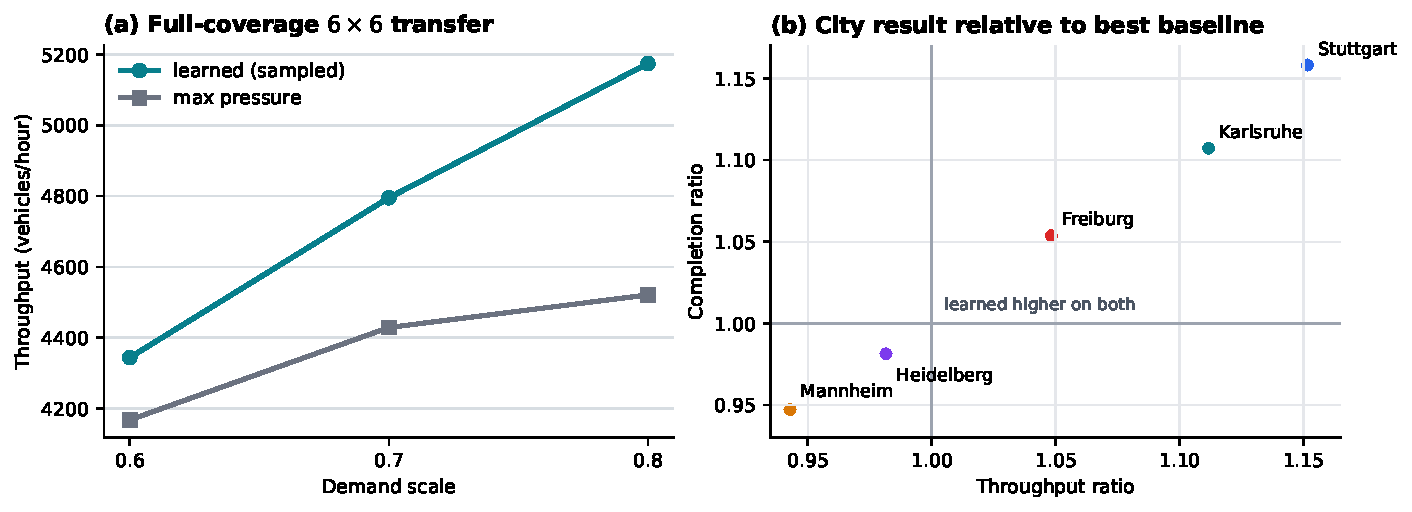
\includegraphics[width=\linewidth]{figures/evaluation-summary.pdf}
  \caption{Observed feasibility results. Left: sampled \(6\times6\) performance over three training seeds and six fresh traffic seeds per demand. Right: iteration-60 city outcomes relative to the highest-throughput baseline listed above, from one training run and three traffic seeds per city.}
  \label{fig:results}
\end{figure}
\FloatBarrier

\textbf{RQ1 --- structural applicability.}
Equations~\eqref{eq:movement-update}--\eqref{eq:lane-update} use shared parameter shapes and return one scalar for every Movement presented to them.
Every junction may independently provide \(A_j\) with its own numbers of rows and columns; phase construction is outside the GNN.
This establishes variable graph and action dimensions by construction.
Execution on graphs ranging from 41 to 84 controlled junctions and phase-count ranges of 2--12 provides an implementation check, not the basis of the property.

\textbf{RQ2 --- synthetic transfer.}
On the unseen-size \(6\times6\) condition, sampled throughput was \(4344,4795,5174\) vehicles/hour at demands \(0.6,0.7,0.8\), versus \(4168,4429,4521\) for max pressure.
Completion was higher in the evaluated runs by \(3.5,6.6,10.6\) percentage points, respectively.
The transposed \(5\times2/2\times5\) and \(5\times3/3\times5\) pairs also had similar observed means.
These findings are consistent with size and aspect-ratio reuse within the matched generator.

\textbf{RQ3 --- distribution shift.}
The full-coverage-trained policy's throughput and completion deteriorated relative to max pressure at \(50\%\) and \(25\%\) signal coverage, despite the graph remaining structurally executable.
In the separate one-seed \(4\times4\) study, a policy trained on \(50\%\)-coverage layouts was close to max pressure under sampled execution at fresh \(25\%\) and \(50\%\) layouts, but its observed throughput and completion were lower at \(75\%\).
The result distinguishes architectural compatibility from robustness and is consistent with sensitivity to the controller-distribution shift.

\textbf{RQ4 --- city feasibility.}
The city evaluation contains one policy-training run; the following values are observations from that run, not estimates of expected cross-city performance.
The trained parameter instance executed without architecture changes on all five city graphs.
Outcomes varied substantially: sampled control had higher throughput and completion than every baseline in Karlsruhe and Stuttgart, trailed queue in Mannheim, was close to fixed time in Heidelberg, and had higher throughput and completion but higher wait density than fixed time in Freiburg.
Across the five equally weighted city means, sampled control observed \(3345.6\) vehicles/hour and \(64.93\%\) completion, versus \(3036.8\) and \(59.37\%\) for max pressure.
This is feasibility evidence from one run.

\section{Limitations and conclusion}

\textbf{Limitations.}
The experiments evaluate the complete implementation and do not isolate individual architectural choices.
In particular, they do not determine the separate contributions of typed relations, two message-passing blocks, or sum-based movement-to-phase aggregation.
The sum aggregation also introduces a phase-size-dependent inductive bias that was not evaluated independently.

The synthetic-grid results concern networks generated by the same underlying process and should not be interpreted as transfer to arbitrary topology.
The signal-coverage study shows that structural compatibility does not imply robustness to changes in the controller distribution.

The city evaluation contains one policy-training seed and three traffic seeds per city.
It shows that one trained parameter instance can execute on several heterogeneous graphs and records the outcomes of that run; it does not estimate expected city-transfer performance.
Similarly, sampled execution performed materially better than greedy execution, so the reported stochastic-policy results should not be treated as evidence for an equivalent deterministic controller.

Finally, the generated phase sets inherit the assumptions and fidelity of the SUMO network and implemented conflict rules.
They are valid action sets under this construction, not formally verified real-world signal plans.

\textbf{Conclusion.}
The implemented interface separates reusable learned scoring from local signal structure: a shared typed GNN emits one scalar per Movement, while deterministic incidence matrices translate those scores into heterogeneous phase spaces.
That separation answers structural applicability by construction.
The experiments add bounded feasibility evidence within synthetic and city simulation families, while the coverage and greedy-execution results show that executable structure alone does not ensure empirical robustness.

\label{lastmainpage}
\clearpage
\bibliographystyle{unsrt}
\bibliography{references}

\clearpage
\appendix
\section{Implementation and scenario details}

\begin{table}[H]
  \centering
  \caption{Anchored training and control settings.}
  \begin{tabular}{@{}lr@{}}
    \toprule
    Setting & Value\\
    \midrule
    Decision interval / yellow & \(5\,\mathrm{s}\) / immediate \(3\,\mathrm{s}\)\\
    Minimum green & one decision\\
    Message-passing blocks / hidden dimension & 2 / 64\\
    Decisions per rollout / PPO epochs & 200 / 4\\
    Entropy coefficient / reward clip & 0.001 / \([-1,1]\)\\
    Progress/discharge/braking/gridlock & \(1/10/10/0.02\)\\
    Global/flow/throughput/switch/teleport weight & 0\\
    Initial occupancy / warm-up & 6--8\% / \(15\,\mathrm{s}\)\\
    \bottomrule
  \end{tabular}
  \label{tab:settings}
\end{table}

\begin{table}[H]
  \centering
  \caption{Structural diversity of the city scenarios. Phase range is the minimum--maximum number of selectable phases per policy-controlled junction.}
  \begin{tabular}{@{}lrrrr@{}}
    \toprule
    City & Controllers & LaneGroups & Movements & Phase range\\
    \midrule
    Karlsruhe & 41 & 286 & 271 & 2--10\\
    Mannheim & 84 & 708 & 467 & 2--7\\
    Stuttgart & 69 & 519 & 508 & 2--12\\
    Heidelberg & 56 & 408 & 365 & 2--10\\
    Freiburg & 58 & 425 & 416 & 2--11\\
    \bottomrule
  \end{tabular}
  \label{tab:city-structure}
\end{table}

\section{Detailed evaluation}

\begin{table}[H]
  \centering
  \caption{Full-coverage \(6\times6\) result. Learned values average three training seeds and six traffic seeds; max pressure averages the six traffic seeds.}
  \begin{tabular}{@{}llrrr@{}}
    \toprule
    Demand & Policy & Throughput/h & Completion & Wait density\\
    \midrule
    0.6 & learned sampled & 4344 & 87.2\% & 0.077\\
        & max pressure & 4168 & 83.6\% & 0.082\\
    0.7 & learned sampled & 4795 & 84.8\% & 0.114\\
        & max pressure & 4429 & 78.2\% & 0.119\\
    0.8 & learned sampled & 5174 & 82.2\% & 0.175\\
        & max pressure & 4521 & 71.5\% & 0.131\\
    \bottomrule
  \end{tabular}
  \label{tab:grid-detail}
\end{table}

\clearpage
\begin{table}[H]
  \centering
  \caption{Iteration-60 city means over three traffic seeds in the single training run. The baseline has the highest throughput among non-learned policies in that city. Wait density is in seconds per metre.}
  \begin{tabular}{@{}llrrr@{}}
    \toprule
    City & Policy & Throughput/h & Completion & Wait density\\
    \midrule
    Karlsruhe & learned sampled & 3452 & 93.86\% & 0.075\\
               & max pressure & 3105 & 84.77\% & 0.243\\
    Mannheim & learned sampled & 3200 & 53.78\% & 0.796\\
              & queue & 3394 & 56.78\% & 1.019\\
    Stuttgart & learned sampled & 4216 & 50.93\% & 0.907\\
               & fixed time & 3661 & 43.97\% & 0.741\\
    Heidelberg & learned sampled & 3190 & 77.69\% & 0.181\\
                & fixed time & 3250 & 79.16\% & 0.127\\
    Freiburg & learned sampled & 2670 & 48.39\% & 1.108\\
              & fixed time & 2547 & 45.92\% & 0.934\\
    \bottomrule
  \end{tabular}
  \label{tab:city-detail}
\end{table}

\paragraph{Sampled versus greedy.}
Across the five equally weighted city means, greedy execution observed \(3182.6\) vehicles/hour, \(61.89\%\) completion, and \(0.980\,\mathrm{s/m}\) wait density, compared with \(3345.6\), \(64.93\%\), and \(0.613\,\mathrm{s/m}\) for sampled execution.
These are descriptive results from the same single training run.

\paragraph{Coverage study.}
The \(50\%\)-coverage training study used one policy-training seed, five training layouts, and three fresh traffic seeds on each of five fresh layouts at \(25\%\), \(50\%\), and \(75\%\) coverage.
For sampled execution, PPO-minus-max-pressure throughput differences were \(+5.7\), \(-28.9\), and \(-104.3\) vehicles/hour; completion differences were \(+0.24\), \(-0.66\), and \(-2.99\) percentage points.
The first two conditions were close in the reported runs; the \(75\%\) observed means were lower.

\paragraph{Evidence granularity.}
Grid means distinguish independent policy-training seeds from traffic seeds.
City and \(4\times4\) coverage results each contain one policy-training seed.
Traffic episodes are therefore repeated simulation observations, not independent learned-policy replications.

\end{document}
